%
% This document contains the chapter about synthesizing circuits.
%
% Copyright (C) 2005, 2006 Stefan Jahn <stefan@lkcc.org>
% Copyright (C) 2005 Michael Margraf <Michael.Margraf@alumni.TU-Berlin.DE>
%
% Permission is granted to copy, distribute and/or modify this document
% under the terms of the GNU Free Documentation License, Version 1.1
% or any later version published by the Free Software Foundation.
%

\chapter{Synthesizing circuits}
\label{sec:synthesis}

\section{Attenuators}

Attenuators are used to damp a signal. Using pure ohmic resistors
the circuit can be realized for a very high bandwidth, i.e. from
DC to many GHz. The power attenuation $0 < L\le 1$ is defined as:
\begin{equation}
\label{eqn:loss}
L = \dfrac{P_{in}}{P_{out}}
  = \dfrac{V_{in}^2}{Z_{in}}\cdot\dfrac{Z_{out}}{V_{out}^2}
  = \left( \dfrac{V_{in}}{V_{out}}\right)^2 \cdot\dfrac{Z_{out}}{Z_{in}}
\end{equation}
where $P_{in}$ and $P_{out}$ are the input and output power and
$V_{in}$ and $V_{out}$ are the input and output voltages.

\begin{figure}[ht]
\begin{center}
\includegraphics[width=5cm]{picircuit}
\end{center}
\caption{$\pi$-topology of an attenuator}
\label{fig:pi_attenuator}
\end{figure}
\FloatBarrier

Fig. \ref{fig:pi_attenuator} shows an attenuator using the
$\pi$-topology. The conductances can be calculated as follows.
\begin{align}
Y_2 & = \dfrac{L - 1}{2\cdot \sqrt{L\cdot Z_{in}\cdot Z_{out}}} \\
Y_1 & = Y_2\cdot\left( \sqrt{\dfrac{Z_{out}}{Z_{in}}\cdot L} - 1 \right) \\
Y_3 & = Y_2\cdot\left( \sqrt{\dfrac{Z_{in}}{Z_{out}}\cdot L} - 1 \right)
\end{align}
where $Z_{in}$ and $Z_{out}$ are the input and output reference
impedances, respectively. The $\pi$-attenuator can be used for an
impedance ratio of:
\begin{equation}
\dfrac{1}{L} \le \dfrac{Z_{out}}{Z_{in}} \le L
\end{equation}

\begin{figure}[ht]
\begin{center}
\includegraphics[width=5cm]{tcircuit}
\end{center}
\caption{T-topology of an attenuator}
\label{fig:t_attenuator}
\end{figure}
\FloatBarrier

Fig. \ref{fig:t_attenuator} shows an attenuator using the
T-topology. The resistances can be calculated as follows.
\begin{align}
Z_2 & = \dfrac{2\cdot \sqrt{L\cdot Z_{in}\cdot Z_{out}}}{L - 1} \\
Z_1 & = Z_{in}\cdot A - Z_2 \\
Z_3 & = Z_{out}\cdot A - Z_2 \\
\textrm{with} \qquad A & = \dfrac{L + 1}{L - 1}
\end{align}
where $L$ is the attenuation ($0 < L\le 1$) according to
equation \ref{eqn:loss} and $Z_{in}$ and $Z_{out}$
are the input and output reference impedance, respectively.
The T-attenuator can be used for an impedance ratio of:
\begin{equation}
\dfrac{Z_{out}}{Z_{in}} \le \dfrac{(L+1)^2}{4\cdot L}
\end{equation}

\section{Filters}

One of the most common tasks in microwave technologies is to
extract a frequency band from others. Optimized filters exist
in order to easily create a filter with an appropriate characteristic.
The most popular ones are:

\addvspace{12pt}

\begin{tabular}{l|l}
Name & Property \\
\hline
Bessel filter (Thomson filter) & as constant group delay as possible \\
Butterworth filter (power-term filter) & as constant amplitude transfer function as possible \\
Chebychev filter type I & constant ripple in pass band \\
Chebychev filter type II & constant ripple in stop band \\
Cauer filter (elliptical filter) & constant ripple in pass and stop band \\
\end{tabular} 

\addvspace{12pt}

From top to bottom the following properties increase:
\begin{itemize}
\item ringing of step response
\item phase distortion
\item steepness of amplitude transfer function at the beginning of the pass band
\end{itemize}

\addvspace{12pt}

The order $n$ of a filter denotes the number of poles of its (voltage)
transfer function. It is:
\begin{equation}
\text{slope of asymptote} = \pm\, n\cdot 20 \text{dB/decade}
\end{equation}
Note that this equation holds for all filter characteristics, but
there are big differences concerning the attenuation near the pass
band.


\subsection{LC ladder filters}

The best possibility to realize a filters in VHF and UHF bands are
LC ladder filters. The usual way to synthesize them is to first
calculate a low-pass (LP) filter and afterwards transform it into a
high-pass (HP), band-pass (BP) or band-stop (BS) filter. To do so,
each component must be transformed into another.

\addvspace{12pt}

In a low-pass filter, there are  parallel capacitors $C_{LP}$ and
series inductors $L_{LP}$ in alternating order. The other filter
classes can be derived from it:

\addvspace{12pt}

In a high-pass filter:
\begin{align}
C_{LP} \quad \rightarrow \quad & L_{HP} = \dfrac{1}{\omega_B^2\cdot C_{LP}} \\
L_{LP} \quad \rightarrow \quad & C_{HP} = \dfrac{1}{\omega_B^2\cdot L_{LP}}
\end{align}

\addvspace{12pt}

In a band-pass filter:
\begin{align}
C_{LP} \quad \rightarrow \quad & \text{parallel resonance circuit with} \\
                               & C_{BP} = \dfrac{C_{LP}}{\Delta\Omega} \\
                               & L_{BP} = \dfrac{\Delta\Omega}{\omega_1\cdot \omega_2\cdot C_{LP}} \\
L_{LP} \quad \rightarrow \quad & \text{series resonance circuit with} \\
                               & C_{BP} = \dfrac{\Delta\Omega}{\omega_1\cdot \omega_2\cdot L_{LP}} \\
                               & L_{BP} = \dfrac{L_{LP}}{\Delta\Omega}
\end{align}

\addvspace{12pt}

In a band-stop filter:
\begin{align}
C_{LP} \quad \rightarrow \quad & \text{series resonance circuit with} \\
       & C_{BP} = \dfrac{C_{LP}}{2\cdot\left| \dfrac{\omega_2}{\omega_1} - \dfrac{\omega_1}{\omega_2} \right| } \\
       & L_{BP} = \dfrac{1}{\omega^2\cdot \Delta\Omega\cdot C_{LP}} \\
L_{LP} \quad \rightarrow \quad & \text{parallel resonance circuit with} \\
       & C_{BP} = \dfrac{1}{\omega^2\cdot \Delta\Omega\cdot L_{LP}} \\
       & L_{BP} = \dfrac{L_{LP}}{2\cdot\left| \dfrac{\omega_2}{\omega_1} - \dfrac{\omega_1}{\omega_2} \right| }
\end{align}

\addvspace{12pt}

Where
\begin{align}
\omega_1 \quad\rightarrow\quad & \text{lower corner frequency of frequency band} \\
\omega_2 \quad\rightarrow\quad & \text{upper corner frequency of frequency band} \\
\omega   \quad\rightarrow\quad & \text{center frequency of frequency band} \quad \omega = 0.5\cdot (\omega_1 + \omega_2) \\
\Delta\Omega \quad\rightarrow\quad & \Delta\Omega = \dfrac{|\omega_2 - \omega_1|}{\omega}
\end{align}

\subsubsection{Butterworth}

The $k$-th element of an $n$ order Butterworth low-pass ladder filter is:
\begin{alignat}{3}
 & \text{capacitance:} \qquad & C_k = & \dfrac{X_k}{Z_0} \\
 & \text{inductance:}  \qquad & L_k = & X_k \cdot Z_0 \\
 & \text{with}         \qquad & X_k = & \dfrac{2}{\omega_B} \cdot \sin \dfrac{(2\cdot k + 1)\cdot\pi}{2\cdot n}
\end{alignat}

The order of the Butterworth filter is dependent on the specifications
provided by the user.  These specifications include the edge
frequencies and gains.
\begin{equation}
\label{eq:ButtOrder}
n = \dfrac{\log{\left(\dfrac{10^{-0.1\cdot \alpha_{stop}} - 1}{10^{-0.1\cdot \alpha_{pass}} - 1}\right)}}{2\cdot\log{\left(\dfrac{\omega_{stop}}{\omega_{pass}}\right)}}
\end{equation}

\subsubsection{Chebyshev I}

The equations for a Chebyshev type I filter are defined recursivly.
With $R_{dB}$ being the passband ripple in decibel, the $k$-th
element of an $n$ order low-pass ladder filter is:
\begin{alignat}{3}
 & \text{capacitance:} \qquad & C_k & = \dfrac{X_k}{Z_0} \\
 & \text{inductance:}  \qquad & L_k & = X_k \cdot Z_0 \\
 & \text{with}         \qquad & X_k & = \dfrac{2}{\omega_B}\cdot g_k \\
 & & r   & = \sinh\left( \frac{1}{n}\cdot\text{arsinh}\dfrac{1}{\sqrt{10^{R_{dB}/10} - 1}} \right) \\
 & & a_k & = \sin \dfrac{(2\cdot k + 1)\cdot\pi}{2\cdot n} \\
 & & g_k & =
\begin{cases}
\begin{array}{ll}
  \dfrac{a_k}{r} & \textrm{ for } \quad k=0\\
  \dfrac{a_{k-1}\cdot a_k}{g_{k-1}\cdot \left( r^2 + \sin^2\dfrac{k\cdot\pi}{n} \right)} & \textrm{ for } \quad k\ge 1
\end{array}
\end{cases} \\
 & & X_k & = \dfrac{2}{\omega_B}\cdot g_k
\end{alignat}

The order of the Chebychev filter is dependent on the specifications
provided by the user.  The general form of the calculation for the
order is the same as for the Butterworth, except that the inverse
hyperbolic cosine function is used in place of the common logarithm
function.
\begin{equation}
\label{eq:ChebOrder}
n = \dfrac{\textrm{sech}\left(\dfrac{10^{-0.1\cdot \alpha_{stop}} - 1}{10^{-0.1\cdot \alpha_{pass}} - 1}\right)}{2\cdot\textrm{sech}\left(\dfrac{\omega_{stop}}{\omega_{pass}}\right)}
\end{equation}

\subsubsection{Chebyshev II}

Because of the nature of the derivation of the inverse Chebychev approximation function from the standard Chebychev approximation the calculation of the order \eqref{eq:ChebOrder} is the same.

\subsection{Quarter wavelength filters}

Quarter wavelength filters are based on the fact that short and open $\lambda/4$ stubs are equivalent to series and paralell resonant tanks, respectively. Once given the normalized $g_i$ coefficients of the filter prototype, it is quite straighforward to obtain the impedance of the short/open stubs, depending on the desired filter mask (bandpass/notch). Figure \ref{eq:QWfilter} illustrates the topology of a quarter wavelength filter.\\

\begin{figure}[H]
\centering
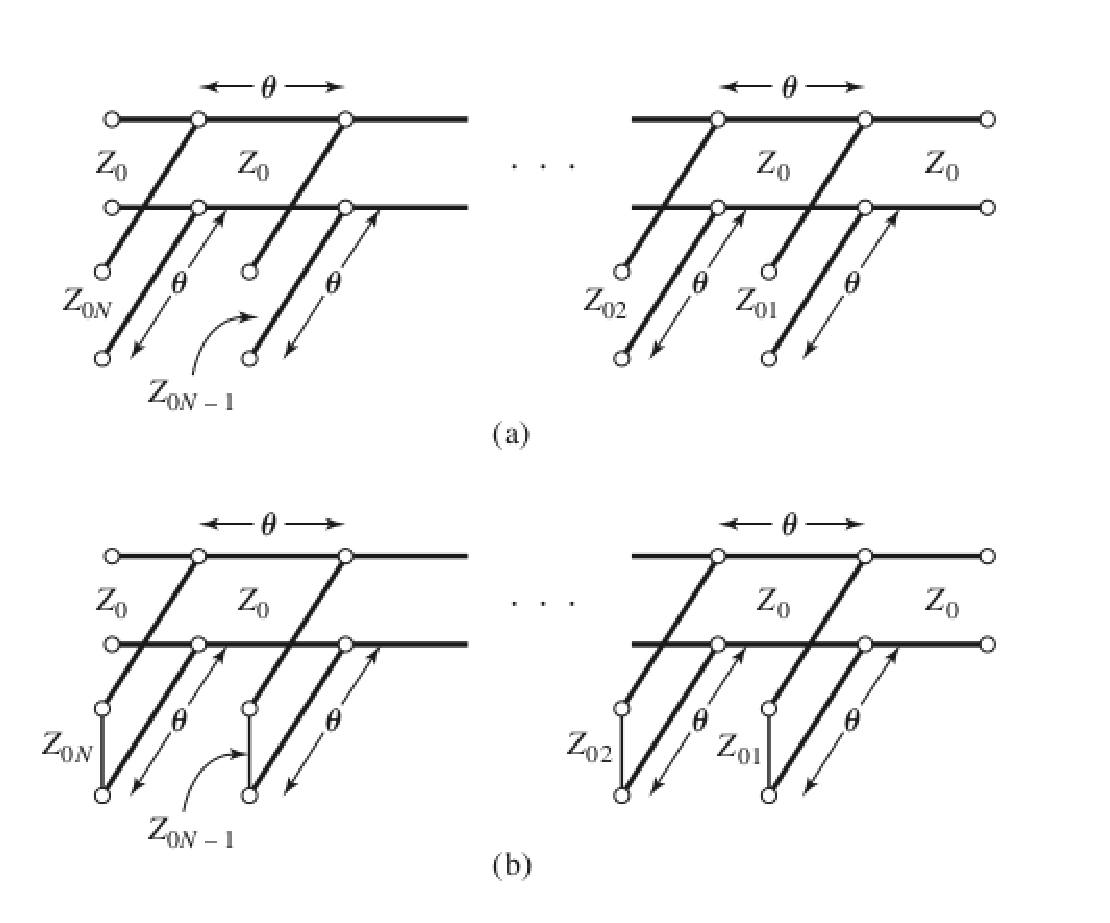
\includegraphics[width=100mm]{QuarterWavelengthFilter.eps}
\caption{Quarter wavelength filters topology. a) Notch filter b) Bandpass filter \cite{Pozar}}
\label{eq:QWfilter}
\end{figure}

\noindent The impedance of the $i$-th stub, $Z_i$, is given by:

\begin{itemize}
\item{Bandpass (short circuit)} $Z_i = \frac{\pi Z_0 \Delta}{4g_i}$
\item{Notch (open circuit)} $Z_i = \frac{4 Z_0 }{g_i\pi \Delta}$
\end{itemize} 

\noindent where $Z_0$ is the characteristic impedance of the filter (typically, 50$\Omega$) and $\Delta$ is the relative bandwidth defined as $\Delta = \frac{f_2 - f_1}{f_c}$. The demonstration \cite{Pozar} is not included in this document in favour of greater simplicity. 

\noindent It has to be said that quarter wavelength filters are narrowband by nature. Besides this, these kind of filters may not be feasible because of the stubs may require unpractical widths (i.e. impedances) for proper operation.

